

\section{Desarrollo}

\subsection{Área de estudio}

Se contaba con datos de ovitrampas de un proyecto proveniente de la Facultad en Oro Verde, para definir el área de interés se llevó a cabo un procesamiento en Python con Folium y Pandas, esto permitió obtener gráficas sobre los puntos geográficos en los que teníamos información de densidad de mosquitos.
	
\begin{figure}[H]
	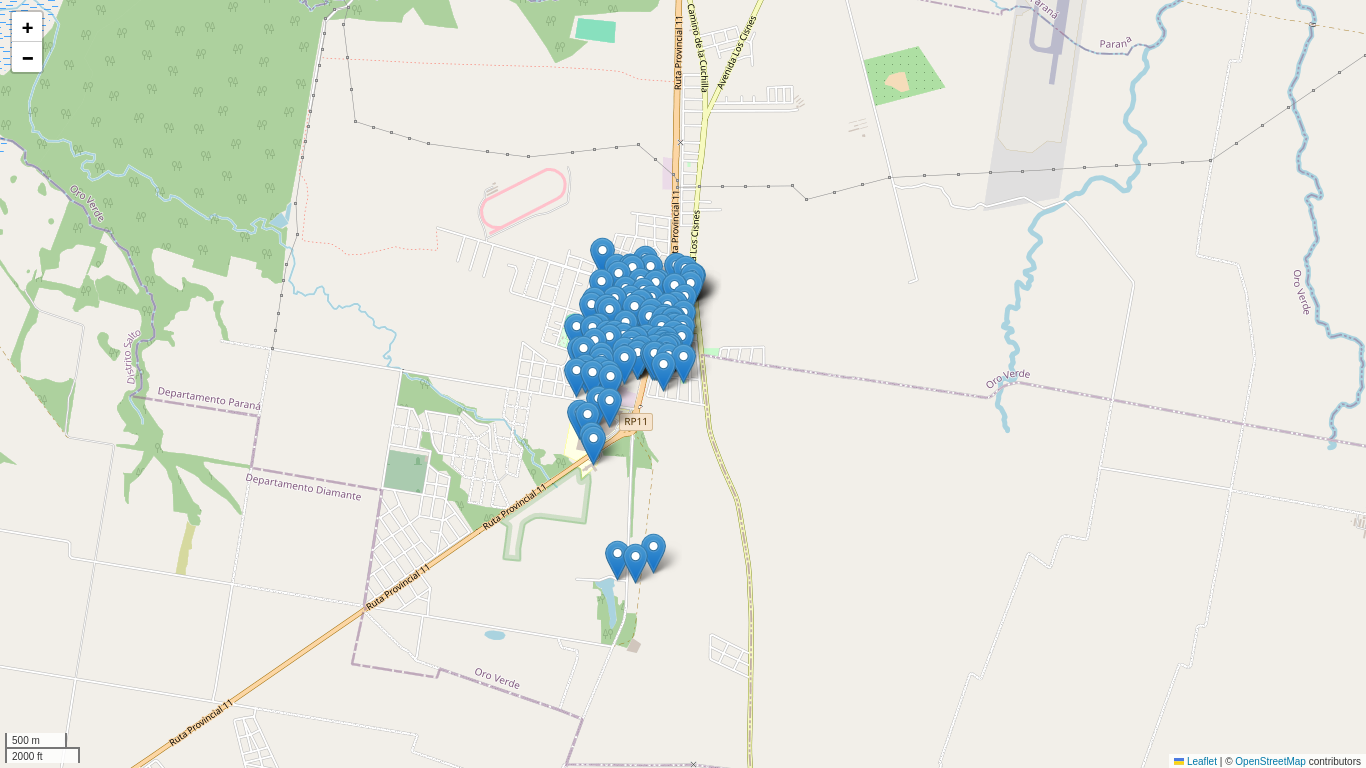
\includegraphics[width=0.7\textwidth]{ovitrampas.png}
	\centering
	\caption{Posiciones de ovitrampas en Oro Verde.}
	\label{fig:ovitrampas}
	
\end{figure}



%% Podría ser buena idea agregar una foto del área de interés desde distintas perspectivas, una en la proyección mundial, otra en el mapa y después directamente la imágen.


\subsection{Obtención de imágenes}

\subsubsection{Dispositivo de sensado}

\subsubsection{Análisis visual}

\subsection{Descripción del modelo}

$$\frac{\partial \rho(P,t)}{\partial t}=\bigtriangledown .(D_R \bigtriangledown \rho)-\bigtriangledown.(\rho D_W V)- \bigtriangledown . (\rho K_H \bigtriangledown H) + \alpha - \beta$$

Donde:

\begin{center}
	\begin{tabular}{|c | c | c|} 
		\hline
		\textbf{Símbolo} & \textbf{Variable} & \textbf{Valor}\\
		\hline
		$$P$$ & Densidad de mosquitos & No homogéneo \\
		\hline
		$\alpha$  & Tasa de nacimientos & $6 (m^2/dia)$ \\
		\hline
		$\beta$  & Tasa de muertes             & 0.2 \\
		\hline
		$V$   & Velocidad Viento Superficie & No homogéneo \\
		\hline
		$K_H$   & Tensor de atracción         & 100 \\
		\hline
		$H$    & Campo de atracción          & No homogéneo \\
		\hline
		$D_R$   & Tensor de difusión          & No homogéneo / ver Tabla 2 \\
		\hline
		$D_W$   & Tensor de rugosidad         & No homogéneo / ver Tabla 2\\
		\hline
	\end{tabular}
\end{center}


